% ---- architecture ~ 4 pages ----

\section{Society Overview}
\label{sec:society}

In this section we present the structure of the agent society and the argumentation framework used in interaction between agents. First our argumentation framework consists of a number of intelligent agents capable of exchanging arguments using the AIF\cite{AIF}. These agents can understand human language and are able to extract arguments from text in English. In addition to the AIF at least one topic ontology is needed in the framework to provide the ground knowledge accepted by all agents in the system. Note that the society is not constrained to use a specific ontology as a whole, but rather each agent needs at least one ontology. This allows agents to play different roles in the society analogous to the roles humans play in our society. For example an agent may have several ontologies describing legal concepts, while other agent may only know about animals. In this approach ontologies shared by all agents represent a limited form common sense knowledge. As we will see in section[\ref{sec:application}] the framework can be augmented with additional capabilities to retrieve data from external sources and insert it into AIF. 

Humans can also take part in a debate using English language. A human can debate on a given topic with one or more agents. As shown in section[\ref{sec:application}] each agent has it's own behavior and different agents may accept different arguments as valid based on their knowledge and various behavior parameters. In a debate each agent maintains an own view of the argumentation and will try at best to attack and defend arguments based on it's own position in the debate. If an agent can't determine the acceptability of an argument he may ask other agents. This is a two step process involving a query to the Facilitator  which returns a list of agents discussing on a given topic. In the next step a query is sent to all agents that might know about this argument. If an agent knows the accessibility value of the property of the argument than an additional query can be made for an argumentation schema. This process may continue in a manner similar to a backward-chaining proof. Note that this process involves agents that share at least one ontology, other than AIF. Because of this agents may form interest groups in the society and interactions only occur within these groups.

\section{Agent Architecture}
\label{sec:application}

In this section we present the architecture of the agent. Each agent can understand natural language and interact with humans and other agents. The NLP module is used to create a schema of argumentation from the text. This schema is used by the reasoning module to determine the argumentation plan and the admissibility of arguments using Dung acceptability. Each agent has also an associated behavior that is essentially a set of parameters that control the algorithms used in the reasoning module. Finally each agent has a communication module used to interact with other agents as described in section[\ref{sec:society}].
Although the use of an ontology has many advantages over other sources of information, such a database or a knowledge base the AIF does not enforce the structure of the domain knowledge used by agents. Because of this any agent can be augmented with capabilities for extracting knowledge. This can be used to support the admissibility of arguments.
In this section we present the architecture of the agent. At the top level we have build an autonomous intelligent agent that has it's own behavior module and reasoning capabilities. Moreover each agent can understand natural language and interact with humans and other agents.
\begin{figure}[t]
\centering
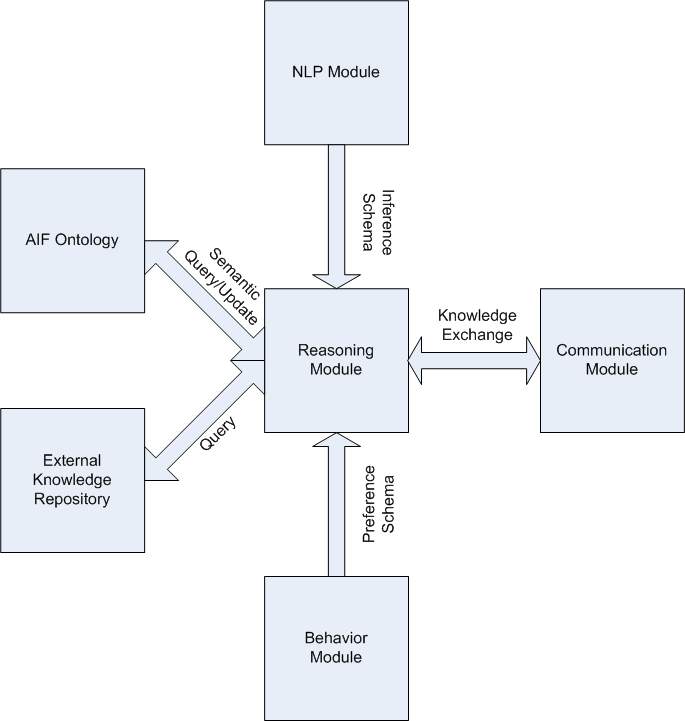
\includegraphics[scale=0.47]{images/TopLevelAgentStructure}
\caption{}
\label{fig:}
\end{figure}

\subsection{NLP Module Description}

The NLP (Natural Language Processing) module is an important component of the overall agent architecture. Its role gains significant attention in the scenario where a human counterpart is engaged in a debate with one or several agents.
In such a setting, the human counterpart will communicate with the agent system using the English language. An individual engaged in a debate will enter text that defines his current standpoint in the entire argumentation process.
The purpose of the NLP module then becomes that of parsing this text and of producing an internal representation of the current argument intended by the user. The output of the module will consist in an inference scheme which will be used by
the main reasoning module of each agent to update its current beliefs and behavior (the way in which it will possibly try to being a counter-argument).

\begin{figure}
\includegraphics[scale=0.5]{images/"NLP Architecture".png}
\caption{Representation of the submodules contained in the NLP component}
\label{fig:NLPArchitecture}
\end{figure}

Figure \ref{fig:NLPArchitecture} shows the general architecture of the NLP module. A description of each module will be given next.

\subsubsection{Argument Identification Module}
\par
The Argument Identification Module classifies all sentences into argumentative and non-argumentative utterances. This module's essential role is to determine which parts of the text are also parts of argument structures.
This module will use a classifier in order to extract argumentative sentences from the input text. 

\par
Our approach takes two possible implementation options into consideration: a naive Bayes classifier and a maximum-entropy method. Regardless of the classifier used, the following list gives a short overview of the features
we intend to use in order to discriminate between argumentative and non-argumentative clauses.

\begin{itemize}
\item Punctuation: The sequence of punctuation marks present in the sentence is used as a feature (e.g. ``:.''). When a punctuation mark occurs more than once in a row, it is considered the same pattern (e.g. two or more successive commas both result in ``,+'').
\item Modal auxiliary: Indicates if a modal auxiliary is present using a POS tagger.
\item Verbs: Detected with a POS tagger. Only the main verbs (excluding ``to be'', ``to do'' and ``to have'') are considered.
\item Adverbs: Detected with a part-of-speech (POS) tagger (e.g. QTag 1).
\item Key words:  Keywords refer to several words or word sequences obtained from a list of terms indicative for argumentation. Examples from the list are ``but'', ``consequently'', and ``because of''.
\end{itemize}

The module will produce an output consisting of a set of sentences deemed as being argumentative. This set will be given as input to the segmentation module described next.

\subsubsection{Segmentation Module}
\par
The Argumentation Identification Module uses this module to partition different argumentative sentences (units) into their corresponding arguments, that is, to determine the limits of each individual argument.
\par
In order to achieve this we opt to calculate the semantic distance between the different argumentative units, and group sentences in one argument if they discuss content that is semantically related. As in the work of Palau and Moens\cite{Palau}, we assume that the relatedness of two sentences is a function of the relatedness of their words.
\par
Given this assumption we take the semantic relatedness of words to be given by their semantic distances in a lexico-semantic resource such as WordNet. We consider the use of three potential word similarity measures.
They are all based on the information content of the least common subsumer (LCS)
of concepts A and B. Information content is a measure of the specificity of a concept, and the LCS of concepts A and B is the most specific concept that is an ancestor of
both A and B. These measures include res (Resnik, 1995)\cite{Resnik}, lin (Lin, 1998)\cite{lin}, and jcn (Jiang and Conrath, 1997)\cite{jcn}.
The lin and jcn measures augment the information content of the LCS with the sum of the information content
of concepts A and B themselves. The lin measure scales the information content of the LCS by this sum, while jcn takes the difference of this sum and the information content of the LCS.
The default source for information content for concepts is the sense-tagged corpus SemCor.

\par
Using these measures we can compute an overall semantic relatedness of the argumentation units. By means of a hierarchical clustering algorithm that will use the distances given by the above mentioned methods we can then segment sentences
into their corresponding arguments (clusters), thus finding the intended argument limits. The hierarchical clustering algorithm computes a dendrogram (a tree like structure) of its given elements. Using an empirically computed threshold, we will cut
the tree at the given depth, thus finding the appropriate sentence clusters.

\subsubsection {Argumentation Scheme Library}
\par
The Argumentation Scheme Library contains abstract forms of argument that capture patterns of reasoning. Each argumentation scheme describes the relations between internal parts (the premises and the conclusion) of a complex argument and, also, the set of critical questions that may attack that argument. Chris Reed and Douglas Walton\cite{reedwalton}, in their research report ``Towards a Formal and Implemented Model of Argumentation Schemes in Agent Communication'' describe the conventional techniques to handle the structure of argumentation schemes in such way that agents may use them in reasoning and also that communication structures can be built around those schemes.
\par
Example of Argumentation Scheme - Argument from Position To Know:
\begin{itemize}
\item Major Premise: Source \emph{a} is in a position to know about things in a certain subject domain \emph{S} containing proposition \emph{A}.
\item Minor Premise: \emph{a} asserts that \emph{A} (in Domain \emph{S}) is true (false).
\item Conclusion: \emph{A} is true (false).
\end{itemize}

This type of argument is defeasible by questioning. Matching the argument from position to know are three critical questions:
\begin{itemize}
\item CQ1: Is \emph{a} in a position to know whether \emph{A} is true (false)?
\item CQ2: Is \emph{a} an honest (trustworthy, reliable) source?
\item CQ3: Did \emph{a} assert that \emph{A} is true (false)?
\end{itemize}
\par
Our Argumentation Scheme Library will be trained from Araucaria DB, which contains several real instantiations of argumentation schemes. The representation used is Argument Markup Language, based upon the industry standard XML.

\subsubsection{Argument Structure Module}
\par
The Argument Identification Module and Segmentation Module were used to distinguish between argumentative and non-argumentative sentences and to group argumentative sentences together into their corresponding argument.
\par
The purpose of this module thus becomes to determine the internal structure of an argument, i.e. the organization of its clauses into conclusions and supporting premises. 
\par
We will consider two possible approaches for this task.
\par
The first relies again on work done by Palau and Moens\cite{Palau} in Argumentation Mining: The Detection, Classification and Structuring of Arguments in Text and considers the partition of an argument's units into premises or conclusions.
\par
For each argument, certain features will be determined. The list can comprise features such as:
\begin{itemize}
\item Tense of Main Verb: Tense of the verb from the main clause of the sentence; having as nominal values ``Present'', ``Past'' or ``No Verb''.
\item History: The most probable argumentative category of previous and next sentence.
\item Rhetorical Patterns: Type of rhetorical pattern occurring on current, previous and next sentences (e.g. ``however,'')
\item Argumentative Patterns: Type of argumentative pattern occurring in sentence
\end{itemize}
A SVM (Support Vector Machine) based algorithm that uses these features will then be used to classify the sentences of an argument into either premises or conclusions.
\par
The second approach is an extension of the first one. Rather than just distinguishing between premise and conclusion, this approach tries to map the argument's structure onto one or several argumentation schemes. 
\par
The definition and format of these schemes is provided by the Argumentation Scheme Library module. 
\par
Making use of more extended features, that will also include the ones listed above, our SVM based algorithm will this time be trained to distinguish between different argumentation schemes. 
